\documentclass[14pt]{beamer}
\usetheme{default}
\usepackage[L7x,T1]{fontenc}
\usepackage[lithuanian]{babel}
\usepackage{graphics}
\usepackage{array}
\usepackage{verbatim}
\usepackage{hyperref}
\usepackage{biblatex}
\usepackage{tabularx}
\usepackage{soul}
\usepackage{mdframed}
\usepackage{tikz}
\usepackage{adjustbox}
\usepackage{mathtools}
\usepackage{caption}
\usepackage{fancyvrb}
\usepackage{subcaption}
\captionsetup{compatibility=false}
\usetikzlibrary{arrows,decorations.pathmorphing,backgrounds,positioning,fit,petri}
\definecolor{vulightgrey}{RGB}{220,220,220}
\definecolor{vupurple}{RGB}{123,0,63}
\definecolor{darkgreen}{RGB}{32,96,32}
\setbeamercolor{title}{fg=vupurple}
\setbeamercolor{frametitle}{fg=vupurple}
\setbeamercolor{item}{fg=vupurple}
\setbeamercolor{navigation symbols dimmed}{fg=vulightgrey}
\setbeamercolor{navigation symbols}{fg=vulightgrey}

\hypersetup{linkcolor=}
\hypersetup{urlcolor=vupurple} % Does not apply color to href's
\hypersetup{colorlinks,urlcolor=vupurple} % href's are correct, but navigation links are magenta

\newcommand{\DP}{Douglas \& Peucker}
\newcommand{\VW}{Visvalingam--Whyatt}
\newcommand{\WM}{Wang--M{\"u}ller}

\mode<presentation>{
    \setbeamertemplate{navigation symbols}{
        \insertslidenavigationsymbol
        \insertframenavigationsymbol
        \hspace{0.2cm}
        \begin{minipage}[c]{0.5cm}
            \vspace{-0.1cm}
            {\strut\insertframenumber{}/\inserttotalframenumber\strut}
        \end{minipage}
    }
}

\iffalse
\setbeamertemplate{footline}[text line]{%
\parbox{\linewidth}{
\vspace*{-8pt}\color{gray}
\textcircled{c}~2016. Uber Technologies Inc. All rights reserved.
}}
\fi

\newcommand{\twocols}[2]
{
    \begin{columns}[c]
        \begin{column}{0.5\textwidth}
            #1
        \end{column}
        \hspace{0pt} \vrule{}
        \begin{column}{0.5\textwidth}
            #2
        \end{column}
    \end{columns}
}

\newcommand{\framedgraphic}[2] {
    \begin{frame}{#1}
        \begin{center}
            \includegraphics[width=\textwidth,height=0.8\textheight,keepaspectratio]{#2}
        \end{center}
    \end{frame}
}

\newcommand{\withcredits}[3]
{
    \begin{minipage}[t][#1\textheight]{\textwidth}
        \vspace{5px}
        #2
    \end{minipage}
    \vfill
    \color{white}{\tiny Šaltinis: #3}
}

%% =============================================================================

\title{
    Kartografinis upių generalizavimas naudojant atvirai prieinamus įrankius
}
\author{Motiejus Jakštys \\
    
\includegraphics[height=10em]{../../misc/Logo_vilniaus_universitetas}
}

\begin{document}

\AtBeginSection[]
{
  \begin{frame}
    \frametitle{Turinys}
    \tableofcontents[currentsection]
  \end{frame}
}

\begin{frame}
\titlepage
\end{frame}

\section{Problema}

\begin{frame}{Kas yra kartografinė generalizacija?}
    \begin{itemize}[<+->]
        \item Mažinant mastelį reikia mažinti detalumą.
        \item Detalumo mažinimas yra sudėtinga problema.
    \end{itemize}
    \onslide<+->{Paimkime pavyzdį.}
\end{frame}

\begin{frame}{Žeimena ir Lakaja}
    \twocols
    {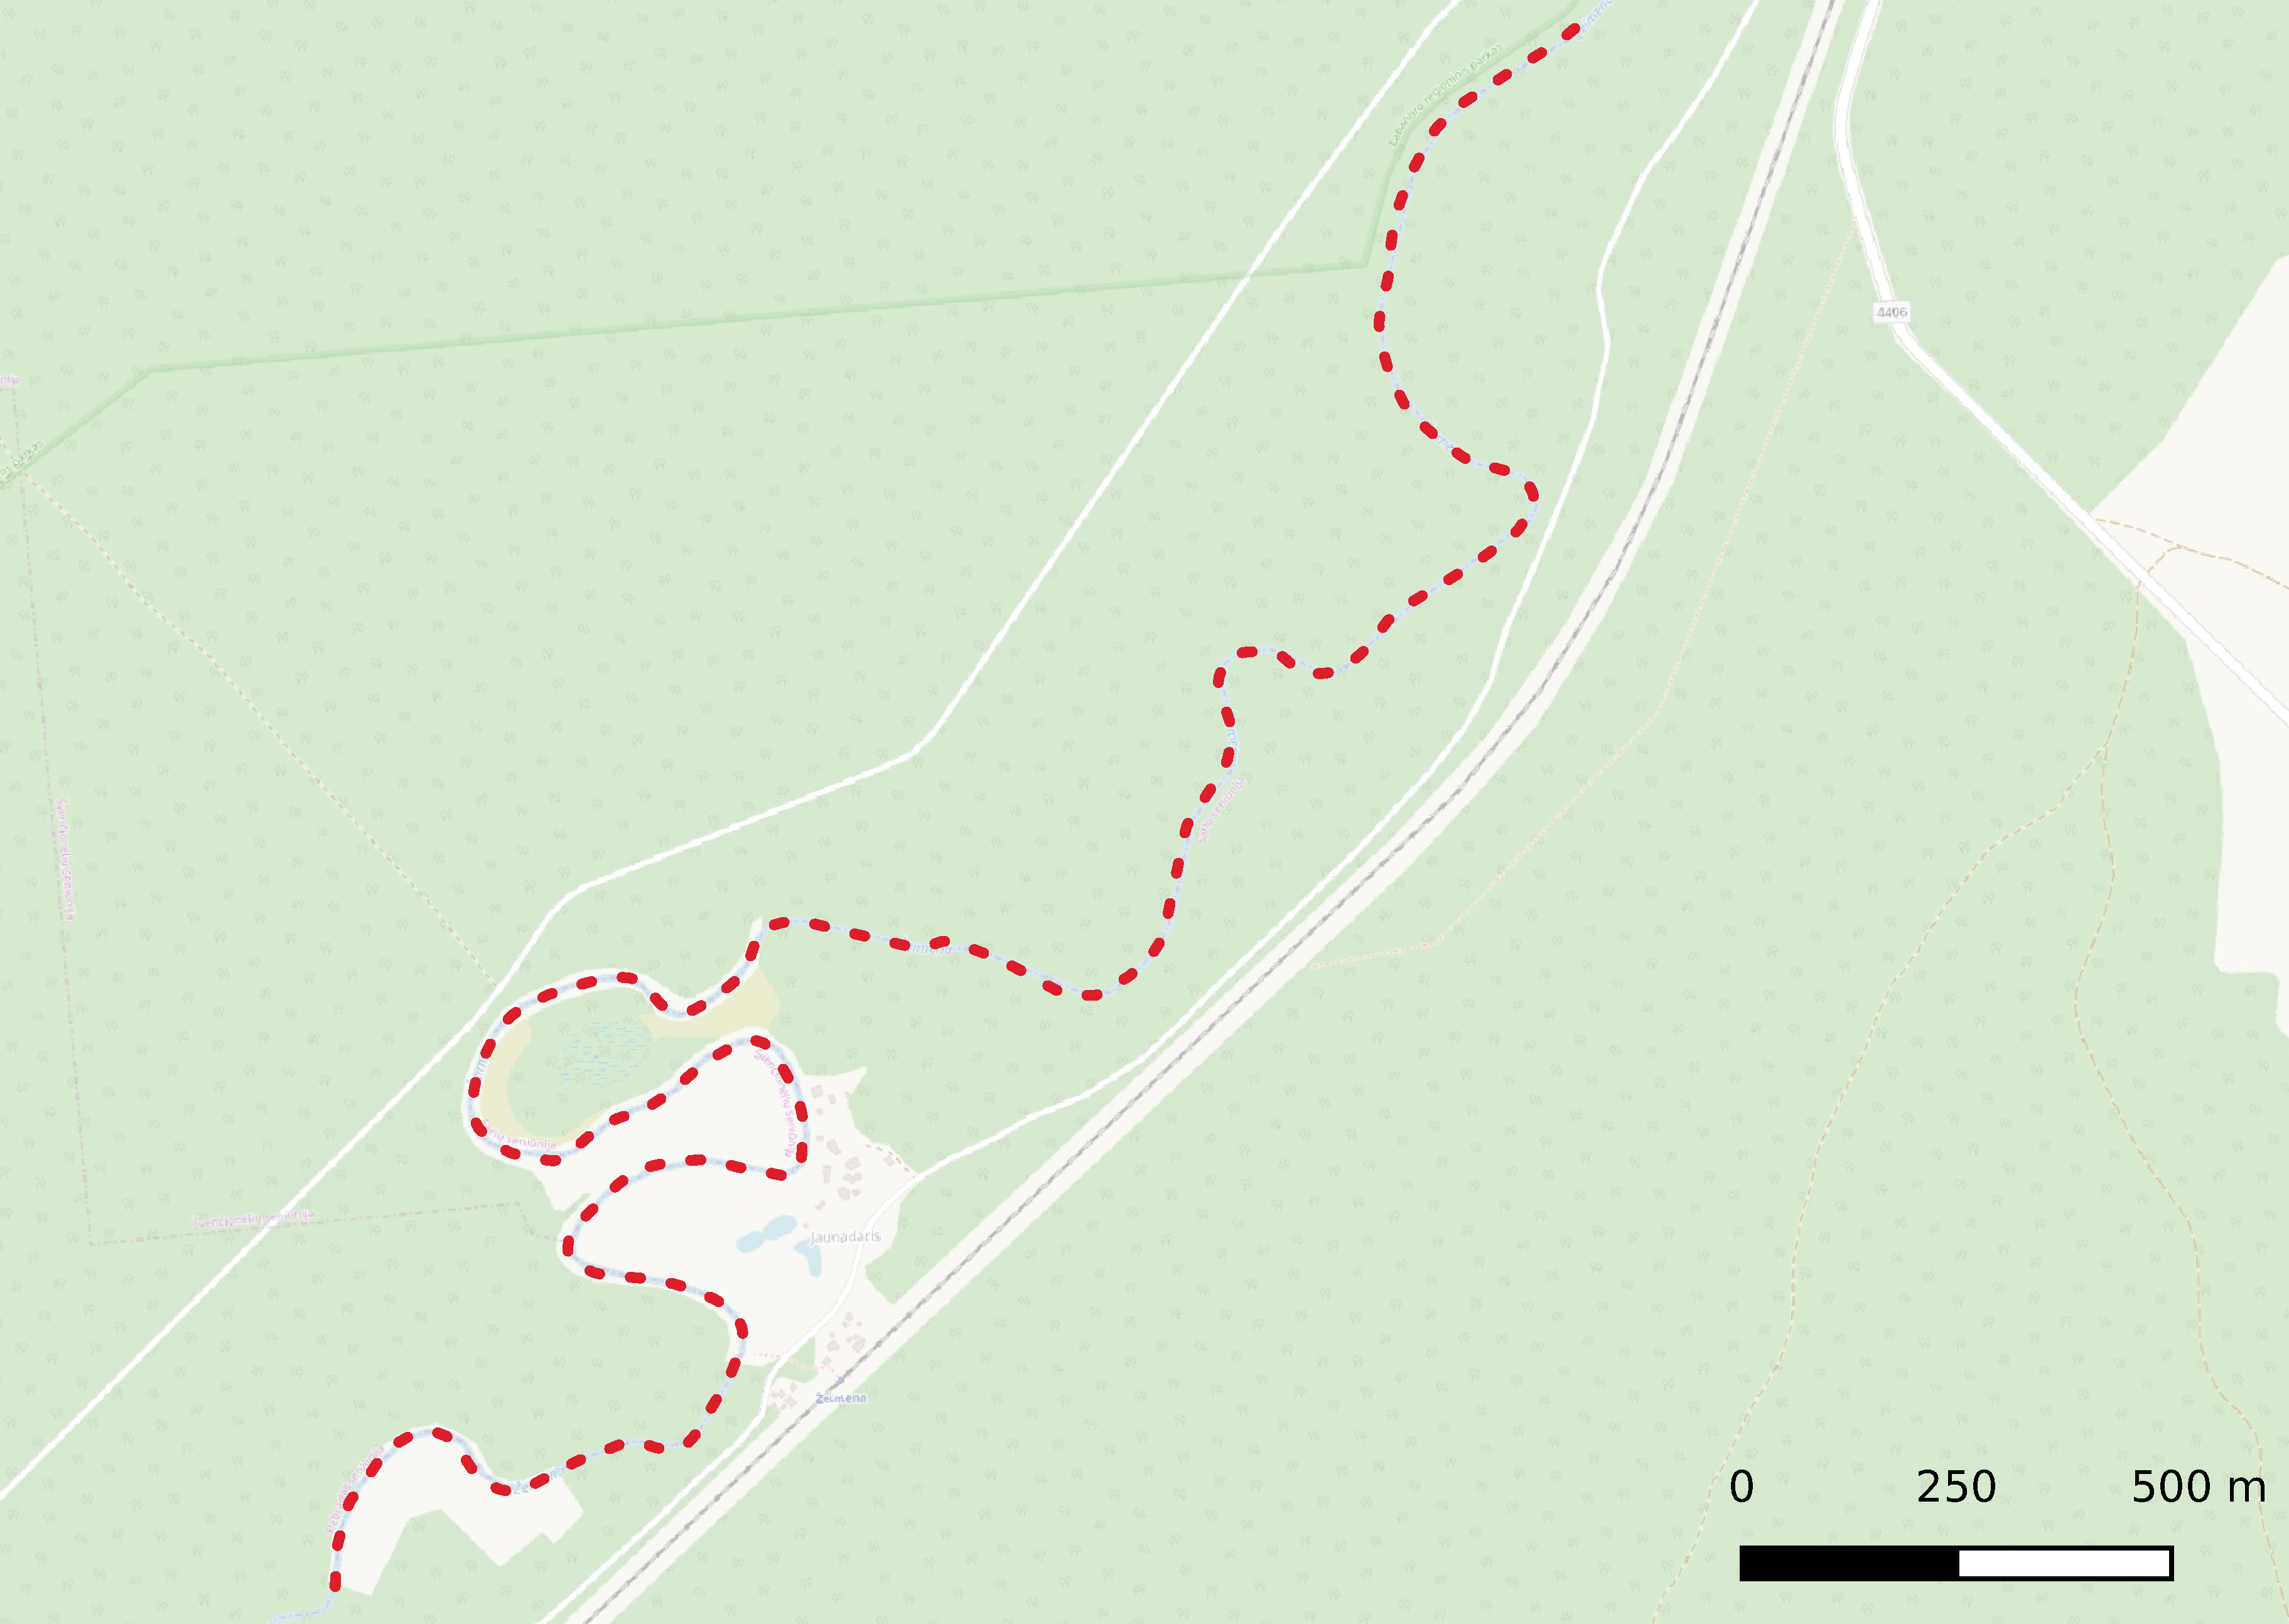
\includegraphics[width=\textwidth]{zeimena}}
    {\includegraphics[width=\textwidth]{crossing}}
\end{frame}

\begin{frame}{Kas yra prieinama?}
    \pause
    \begin{itemize}[<+->]
        \item Atvira ir galima naudoti:
            \begin{itemize}[<+->]
                \item {\DP}
                \item {\VW}
            \end{itemize}
        \item Komerciniame produkte:
            \begin{itemize}[<+->]
                \item {\WM}
            \end{itemize}
    \end{itemize}
\end{frame}

\begin{frame}{Pritaikant dabartinius algoritmus}
    \pause
    \begin{tabularx}{\textwidth}{ | X | X | }
        Douglas \& Peucker                                                   &
        Visvalingam-Whyatt                                                   \tabularnewline \hline

        \onslide<3->{\center
            \includegraphics[width=.75\linewidth]{overlaid-zeimena-douglas-64}}      &
        \onslide<3->{\center
            \includegraphics[width=.75\linewidth]{overlaid-zeimena-visvalingam-64}}  \tabularnewline \hline

        \onslide<4->{\center
            \includegraphics[width=.75\linewidth]{overlaid-zeimena-douglas-256}}     &
        \onslide<4->{\center
            \includegraphics[width=.75\linewidth]{overlaid-zeimena-visvalingam-256}} \tabularnewline \hline
    \end{tabularx}
\end{frame}

\begin{frame}{Problemos}
    Ne taip, kaip kartografai generalizuotų:
    \pause
    \begin{itemize}[<+->]
        \item Daug "kampų" ir "dantų".
        \item Nedideli vingiai visiškai dingsta.
        \item Upės beveik niekada nebūna tiesios.
    \end{itemize}
\end{frame}


\section{Pasiūlymas}

\begin{frame}{Algoritmas}
    \begin{center}
        \fbox{
            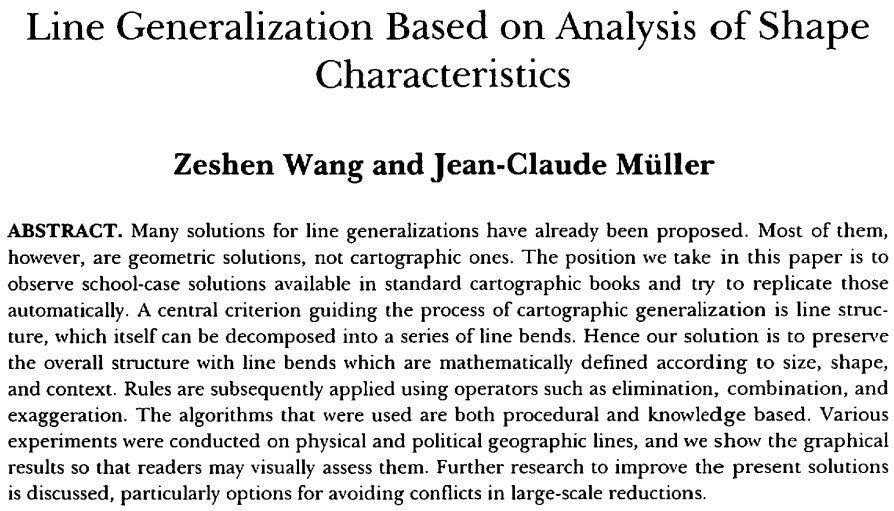
\includegraphics[width=\textwidth]{images/wang1998line.png}
        }
    \end{center}
\end{frame}

\begin{frame}{Pagrindiniai privalumai}
    Sukurtas pagal tai, kaip kartografai generalizuotų:
    \pause
    \begin{itemize}[<+->]
        \item Nesukuriami "kampai" ir "dantys".
        \item Nedideli vingiai "prastinami" į vieną didesnį.
        \item Nesukuria tiesių upių.
    \end{itemize}
\end{frame}

\begin{frame}{Technologijos}
    \begin{itemize}[<+->]
        \item {\texttt qgis.core}
        \item PostGIS 3.x
    \end{itemize}
\end{frame}

\section{Darbo eiga}

\begin{frame}{Darbo eiga}
    \begin{itemize}[<+->]
        \item Parašyti algoritmą.
        \item Aprašyti rezultatus.
    \end{itemize}
\end{frame}

\end{document}
